\documentclass[tikz,border=4pt]{standalone}
\usepackage{amsmath}
\begin{document}
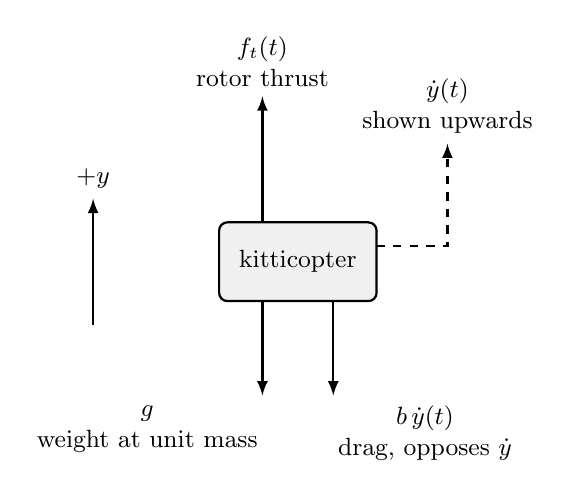
\begin{tikzpicture}[>=latex,thick,font=\small]
  % body
  \draw[rounded corners=3pt,fill=gray!12] (-1.0,-0.5) rectangle (1.0,0.5);
  \node at (0,0) {kitticopter};

  % thrust, up
  \draw[->] (-0.45,0.5) -- (-0.45,2.1) node[above,align=center] {$f_t(t)$\\rotor thrust};

  % drag, down for an upward velocity
  \draw[->] (0.45,-0.5) -- (0.45,-1.7) node[below right,align=center,xshift=-2pt]
    {$b\,\dot{y}(t)$\\drag, opposes $\dot{y}$};

  % weight, down
  \draw[->] (-0.45,-0.5) -- (-0.45,-1.7) node[below left,align=center,xshift=2pt]
    {$g$\\weight at unit mass};

  % velocity shown as the case the drag sign is drawn for
  \draw[->,dashed] (1.0,0.2) -- (1.9,0.2) -- (1.9,1.5) node[above,align=center] {$\dot{y}(t)$\\shown upwards};

  % sign convention
  \draw[->] (-2.6,-0.8) -- (-2.6,0.8) node[above] {$+y$};
\end{tikzpicture}
\end{document}
